\section{Background}  
Secure communication over the Internet has long relied on the interplay between protocols that guarantee reliability and those that ensure privacy. Historically, this has been achieved through the layered combination of TCP (Transmission Control Protocol) and TLS (Transport Layer Security) - a partnership that prioritizes backward compatibility and incremental evolution. In contrast, QUIC (Quick UDP Internet Connections) represents a paradigm shift, integrating transport and security into a unified protocol designed for the demands of modern networks. Understanding their architectural philosophies is key to evaluating their performance and security trade-offs.

\subsection{The Layered Approach: TCP + TLS}
TCP, the bedrock of Internet communication since the 1970s, was designed to solve a fundamental problem: how to reliably transmit data across inherently unreliable networks \cite{postel1981rfc0793}. By establishing connections through its three-way handshake, enforcing in-order packet delivery, and dynamically adjusting transmission rates via congestion control algorithms like Cubic and BBR \cite{allman2009tcp, cardwell2016bbr}, TCP ensures that data arrives intact and sequenced. However, this reliability comes at a cost. For instance, TCP's strict in-order delivery creates head-of-line blocking, where a single lost packet stalls all subsequent data, a bottleneck even more relevant in high-latency or lossy environments like mobile networks.
 
To address TCP's lack of inherent security, TLS emerged as a cryptographic layer operating on top of it. TLS 1.3, the latest iteration, streamlines the handshake process to a single round trip (or zero for resumed connections) and employs modern encryption suites like AES-GCM and ChaCha20-Poly1305. Yet, because TLS operates as a separate layer, establishing a secure connection requires sequential handshakes: first TCP negotiates the transport channel, then TLS authenticates and encrypts it. For a new connection, this results in 2.5 round trips of latency before any application data is transmitted - a delay that effects in global-scale systems where round-trip times often exceed 100 milliseconds.

This layered design, while modular and backward-compatible, introduces inefficiencies. Middle entities like firewalls and NATs \cite{langley2017quic}, optimized for decades of TCP traffic, often misinterpret or hinder TLS-specific optimizations. Moreover, TCP's head-of-line blocking persists even after TLS encrypts the data, as packet loss at the transport layer stalls the entire encrypted stream. These limitations motivated the search for a protocol that could reimagine both transport and security as a whole.

\begin{figure}[!b]
	\centering
	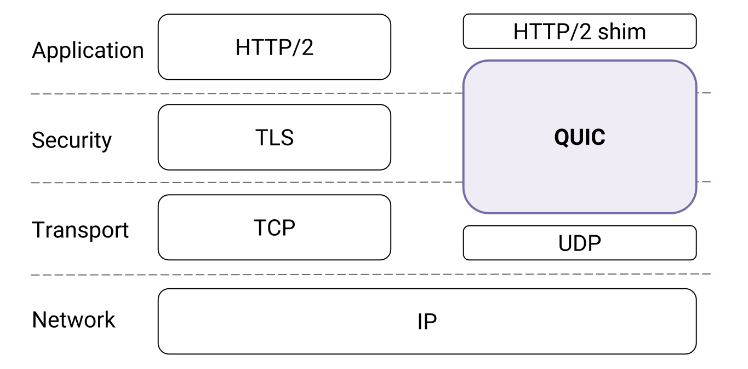
\includegraphics[width=0.65\textwidth]{images/quic-stack.png}
	\caption{QUIC in the traditional HTTPS stack \cite{langley2017quic}.}
\end{figure}

\subsection{QUIC}
QUIC, first deployed by Google in 2012 and later standardized as the foundation of HTTP/3, challenges the layered approach of TCP + TLS. Built on top of UDP, a protocol without built-in reliability or congestion control, QUIC integrates transport and cryptographic handshakes into a single layer. This integration reflects a design philosophy where security is mandatory, latency is minimized, and reliability is redefined for modern use cases.

From its inception, QUIC mandates encryption. Unlike TCP + TLS, where encryption is an optional add-on, QUIC embeds TLS 1.3 directly into its handshake, ensuring that every connection is secured by default. This allows QUIC to merge the transport and cryptographic handshake into 1 round trip for new connections and 0-RTT for resumed sessions. For example, a user resuming a connection on a mobile network could begin transmitting data immediately, avoiding the 200+ milliseconds of handshake latency typical of the traditional stack. QUIC further diverges from TCP through its handling of multiplexing. By allowing multiple independent streams within a single connection, QUIC eliminates head-of-line blocking at the application layer. If a packet is lost on one stream, other streams continue unaffected - a critical advantage for real-time applications. Additionally, QUIC supports connection migration, enabling seamless transitions between networks without renegotiating security parameters, a feature TCP struggles with due to its strict linkage of connection to IP addresses and ports.